% ==============================================================================
% 序幕：如何编程 (Prologue: How to Program)
% ==============================================================================

\chapter{序幕：如何编程}
\renewcommand{\thefigure}{0.\arabic{figure}}\setcounter{figure}{0}
\renewcommand{\thetable}{0.\arabic{table}}\setcounter{table}{0}
\label{sec:prologue}

\begin{center}
  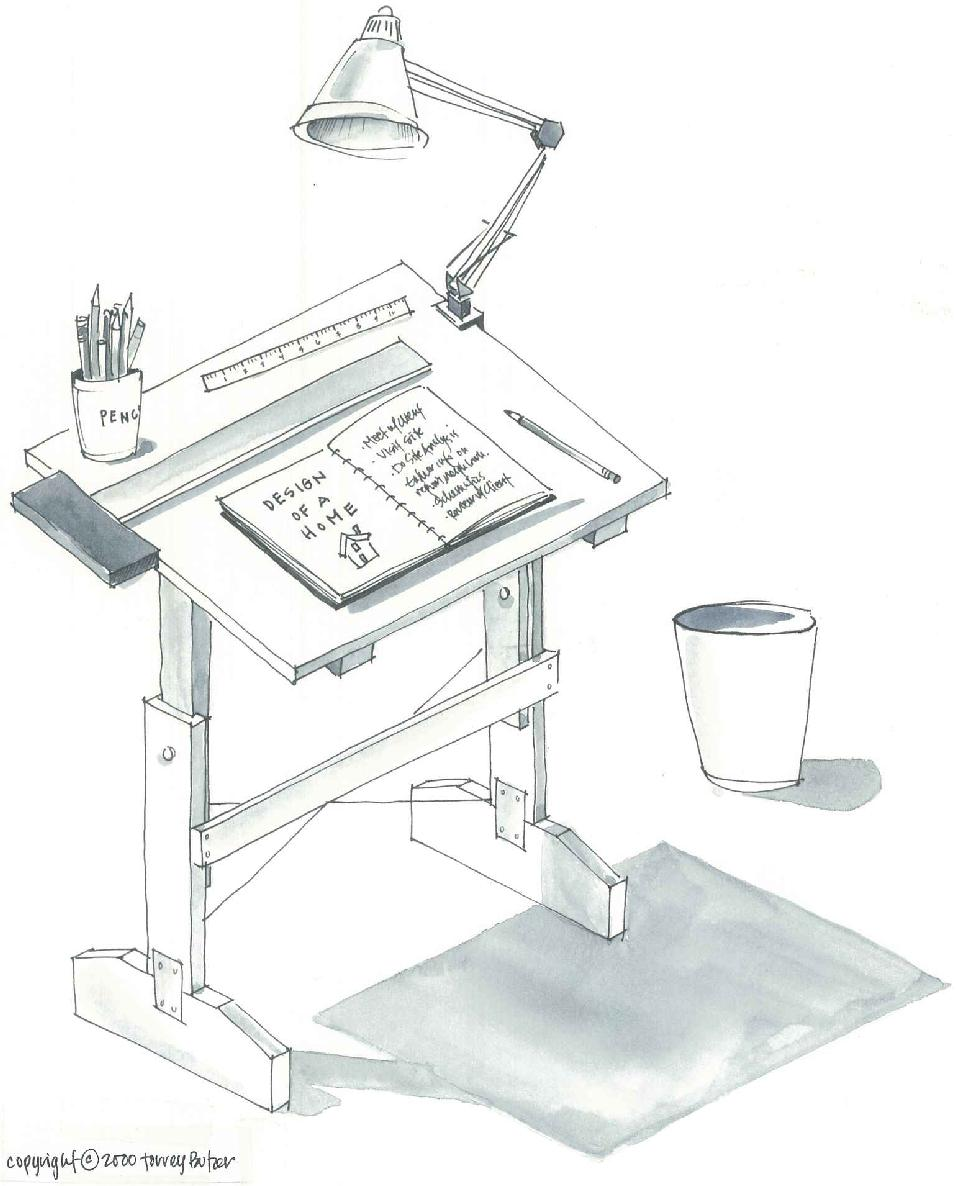
\includegraphics[width=0.45\textwidth]{images/00003.jpeg}
\end{center}

当你还是个幼童时，父母就教你数数，并用手指做简单的算术运算：“1 + 1 是 2”、“1 + 2 是 3”，等等。接着他们会问：“那 3 + 2 是几？”你会掰着一只手的手指头数出答案。他们负责下达指令（编程），你负责执行计算。从某种意义上说，这其实就是“编程”与“计算”的全部实质。

\begin{notebox}[环境准备]
从官方网站下载并安装最新版的 DrRacket 软件：\url{https://racket-lang.org}。
\end{notebox}

现在，是时候互换角色了。启动 DrRacket，你将看到如图~\ref{fig:meet_drracket} 所示的主界面。从顶部的“Language”（语言）菜单中选择“Choose Language...”（选择语言），在弹出的对话框中找到“How to Design Programs”分类下的“Teaching Languages”（教学语言），选择“Beginning Student”（初学学生语言，简称 \term{BSL}），然后点击“OK”完成设置。至此，角色彻底互换：你成为了发号施令的程序员，而 DrRacket 软件则成了那个乖巧听话、为你计算的小朋友。

让我们从最简单的计算开始。在 DrRacket 窗口的上半部分键入：
\begin{lstlisting}[language=BSL]
(+ 1 1)
\end{lstlisting}
点击右上角绿色的“Run”（运行）按钮，窗口的下半部分就会立即显示出一个醒目的结果：\code{2}。

\begin{figure}[htbp]
  \centering
  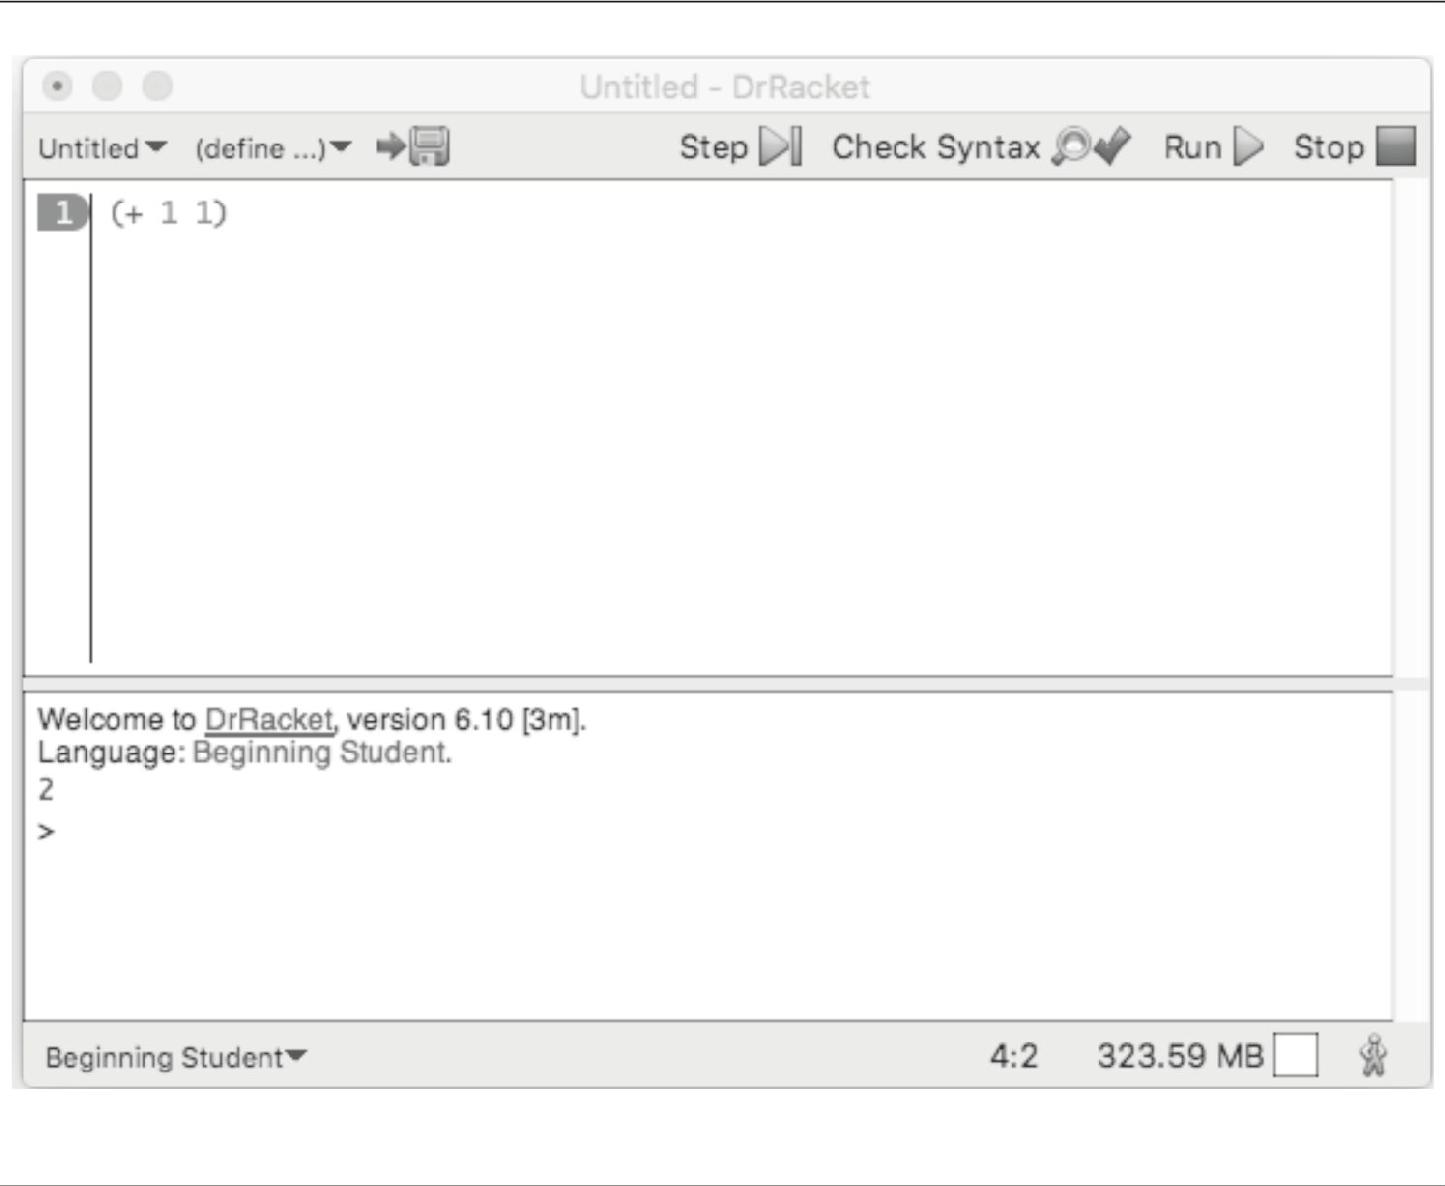
\includegraphics[width=0.9\textwidth]{images/00004.jpeg}
  \caption{初识 DrRacket 编程集成环境}
  \label{fig:meet_drracket}
\end{figure}

编程就是如此轻松直观。你像对待小朋友那样向 DrRacket 发问，DrRacket 为你完成计算。你也可以让 DrRacket 一次性处理多个运算请求：
\begin{lstlisting}[language=BSL]
(+ 2 2)
(* 3 3)
(- 4 2)
(/ 6 2)
\end{lstlisting}
点击“Run”后，DrRacket 的下半部分会依次输出：\code{4}、\code{9}、\code{2}、\code{3}，完全符合你的预期。

让我们放慢脚步，正式引入几个核心概念与专业术语：
\begin{itemize}
  \item DrRacket 窗口的上半部分称为\term{定义区}（definitions area）。在定义区中，你负责创建和修改程序代码，这一过程称为\term{编辑}（editing）。一旦你在定义区输入了字符或作出了任何修改，左上角就会亮起“Save”（保存）按钮。第一次点击“Save”时，DrRacket 会提示你输入文件名，以便将程序安全永久地保存在硬盘上。只要定义区与文件关联，点击“Save”就能确保你的全部心血安全留存。
  
  \item 程序由\term{表达式}（expressions）构成。在数学中你早已熟悉表达式的概念。在目前的 BSL 中，一个表达式要么是一个纯数字，要么是一个以左括号“\code{(}”开头、以匹配的右括号“\code{)}”结尾的括号结构——作为视觉奖励与辅助，DrRacket 会用阴影柔和地高亮配对括号之间的区域。
  
  \item 当你点击“Run”时，DrRacket 会自动对定义区中的所有表达式进行求值，并在下半部分的\term{交互区}（interactions area）中打印出求值结果。随后，DrRacket 作为忠诚的数字助手，在提示符（\code{>}）后静候你的下一步指示。提示符的出现表明 DrRacket 已经准备就绪，等待你在交互区直接输入额外的表达式并实时求值：
  \begin{replbox}
> (+ 1 1)
2
  \end{replbox}
\end{itemize}

在提示符后键入表达式，按下键盘上的回车键（Return / Enter），观察 DrRacket 给出的即时响应。你可以随心所欲地反复尝试：
\begin{replbox}
> (+ 2 2)
4
> (* 3 3)
9
> (- 4 2)
2
> (/ 6 2)
3
> (sqr 3)
9
> (expt 2 3)
8
> (sin 0)
0
> (cos pi)
#i-1.0
\end{replbox}

请格外仔细地观察最后一个结果。其前缀 \code{\#i} 是“我不大清楚绝对精确的值是多少，暂且用这个近似值代表”的缩写，在计算机科学中称为\term{不精确数}（inexact number）。与普通的袖珍计算器或其他编程系统不同，DrRacket 表现得极其诚实：当它无法给出完全精确的数学结果时，便会主动加上这个特殊前缀发出明确警示。在后续的插曲中，我们将为你揭开关于“计算机数字表示”的种种惊人真相，届时你定会由衷赞赏 DrRacket 的诚实与严谨。

此时你可能会好奇，DrRacket 能否一次性将两个以上的数字相加？答案是完全可以，而且有两种不同的写法：
\begin{replbox}
> (+ 2 (+ 3 4))
9
> (+ 2 3 4)
9
\end{replbox}
第一种写法是我们在学校代数课中所熟悉的\textbf{嵌套算术}（nested arithmetic）。第二种写法则是 BSL 原生的\textbf{前缀算术}。后者极为自然，因为在这种记法中，括号始终用来明确地将“运算操作符”与其“操作数”紧密组合在一起。

\begin{notebox}[关于 Racket 的说明]
尽管这个编辑器名为 DrRacket，但本书并不教授 Racket 语言本身。关于为何专为教学研发一套独立的教学语言体系，详见前言中关于教学语言的阐述。
\end{notebox}

在 BSL 中，每次想要执行计算操作时，你先写一个左括号，写下想要执行的操作符（例如 \code{+}），接着写下该操作所作用的各个数值（彼此用空格或换行分隔），最后以一个闭合的右括号结尾。紧跟在操作符后面的项称为\term{操作数}（operands）。所谓嵌套算术，意味着操作数本身也可以是一个表达式，因此：
\begin{replbox}
> (+ 2 (+ 3 4))
9
\end{replbox}
是一个完全合法的优良程序。你可以根据需要任意嵌套：
\begin{replbox}
> (+ 2 (+ (* 3 3) 4))
15
> (+ 2 (+ (* 3 (/ 12 4)) 4))
15
> (+ (* 5 5) (+ (* 3 (/ 12 4)) 4))
38
\end{replbox}
嵌套层数没有任何人为限制，唯一的限制是你的耐心。

自然，当 DrRacket 为你进行计算时，遵循的是你在数学中所熟知且钟爱的经典求值法则：只有当所有操作数都已化简为纯数字时，它才能算出加法的结果。如果某个操作数本身是一个带括号的子表达式，它会优先计算该内层表达式的值。与人类做四则运算不同，DrRacket 永远不需要为“先乘除还是先加减”这类运算符优先级伤脑筋——因为“自内向外”的纯括号求值是这里唯一通行的法则。

这种便利的代价是：\textbf{括号具有严格的语法意义}。你必须输入所有必需的括号，但绝不能输入多余的括号。例如在数学作业中添加多余的外层括号老师通常不会扣分，但在 BSL 中则绝对行不通。\code{(+ (1) (2))} 包含了多余的括号，DrRacket 会毫不客气地给出错误诊断：
\begin{replbox}
> (+ (1) (2))
function call: expected a function after the open parenthesis, found a number
\end{replbox}
不过一旦你习惯了 BSL 编程，就会发现这根本不是什么负担，反而带来了巨大的优势：首先，你可以对任意多个操作数同时施加操作：
\begin{replbox}
> (+ 1 2 3 4 5 6 7 8 9 0)
45
> (* 1 2 3 4 5 6 7 8 9 0)
0
\end{replbox}
如果你不确定某个操作符是否支持多个操作数，只需在交互区输入一个例子并敲击回车；DrRacket 会立刻告诉你它是否可行。或者按下 F1 打开 HelpDesk 查阅文档。其次，在阅读他人编写的程序时，你永远不需要费神去猜想哪个子表达式会优先被求值——清晰的括号与嵌套层次能够瞬间把求值顺序一览无遗地呈现在眼前。

\begin{notebox}[提示]
在在线版教材中，所有操作符的名称都超链接到了 HelpDesk 文档；在 DrRacket 中按 F1 亦可随时查看光标所在词的文档。
\end{notebox}

在此语境下，\term{编程}（programming）就是编写出易于理解的算术表达式，而\term{计算}（computing）就是求出表达式的值。借助 DrRacket，探索这种纯粹的编程与计算变得无比轻松。


% ------------------------------------------------------------------------------
\section{算术与“算术”}
\label{sec:prologue:arithmetic}
% ------------------------------------------------------------------------------

如果编程仅仅局限于枯燥的数字与四则运算，那它未免会像纯粹的初等数学那样单调。所幸的是，编程的世界远比数字丰富得多：文字、真假逻辑、图像以及更多丰富多彩的数据形态。

\begin{notebox}[幽默旁白]
开个玩笑：数学其实是一门极其迷人的学科，只是在当前的编程入门阶段，你并不需要用到高深的数学知识。
\end{notebox}

首先你需要了解的是，在 BSL 中，\term{文本}（text）是由双引号（\code{"}）括起来的任意键盘字符序列。我们将其称为\term{字符串}（string）。因此，\code{"hello world"} 是一个完全合法的字符串；当 DrRacket 对该字符串求值时，它就像对待数字那样，原封不动地在交互区将其回显出来：
\begin{replbox}
> "hello world"
"hello world"
\end{replbox}
事实上，许多程序员人生中写出的第一个程序，就是用来显示这行著名的问候语。

不仅如此，除了针对数字的算术之外，DrRacket 还精通针对字符串的“算术”。以下两个交互示例展示了这种独特的字符串算术：
\begin{replbox}
> (string-append "hello" "world")
"helloworld"
> (string-append "hello " "world")
"hello world"
\end{replbox}
正如 \code{+} 一样，\code{string-append} 也是一个操作符；它通过将后一个字符串拼接到前一个字符串的末尾来生成一个新字符串。正如第一个交互所示，这种拼接是完全原样的，两个字符串之间绝不会自动插入任何空格或标点。因此，如果你想要得到 \code{"hello world"}，就必须在其中一个单词中显式包含空格；这正是第二个交互所呈现的。当然，从两个单词构造该短语最自然的写法是：
\begin{replbox}
> (string-append "hello" " " "world")
"hello world"
\end{replbox}
因为与 \code{+} 一样，\code{string-append} 也能够同时接收任意多个操作数。

对字符串能做的事情远不止拼接。你可以从字符串中截取子串、翻转字符串、将所有字母转换为大写（或小写）、剔除两端的空格等等。最美妙的是，你根本不需要死记硬背这些函数名。只要在 HelpDesk 中检索相关词条，随时都能查到字符串支持的所有操作。

\begin{notebox}[使用 HelpDesk]
在键盘上按下 F1 键或使用顶部的帮助菜单打开 HelpDesk。阅读 BSL 手册中关于预定义操作的章节，特别是针对字符串的丰富操作函数。
\end{notebox}

如果你查阅了 BSL 的内置原语操作，会发现原语操作不仅能够消费字符串，还能生成数字：
\begin{replbox}
> (+ (string-length "hello world") 20)
31
> (number->string 42)
"42"
\end{replbox}
同时，也存在将字符串转换为数字的逆向操作：
\begin{replbox}
> (string->number "42")
42
\end{replbox}
如果你期待输入 \code{"forty-two"} 能得到 42，那可就想多了——这可不是一个严谨的字符串转换函数所能胜任的。

最后一个表达式引发了一个有趣的问题：如果有人将一个内部根本不是数字的字符串传给 \code{string->number}，会发生什么？在这种情况下，该操作会返回一种完全不同形态的结果：
\begin{replbox}
> (string->number "hello world")
#false
\end{replbox}
这既不是数字，也不是字符串，而是一个\term{布尔值}（Boolean）。与无穷无尽的数字和字符串不同，布尔值在全宇宙中只有两种可能取值：\code{\#true} 与 \code{\#false}。前者代表“真”，后者代表“假”。尽管取值只有两个，DrRacket 依然提供了一组专门用于组合布尔值的丰富操作符：
\begin{replbox}
> (and #true #true)
#true
> (and #true #false)
#false
> (or #true #false)
#true
> (or #false #false)
#false
> (not #false)
#true
\end{replbox}
运算结果完全符合操作符名称所传达的逻辑真意。（如果不熟悉 \code{and}、\code{or} 与 \code{not} 的逻辑法则，其实很简单：\code{(and x y)} 当且仅当 \code{x} 与 \code{y} 均为真时才为真；\code{(or x y)} 只要两者中至少有一个为真即为真；而 \code{(not x)} 在 \code{x} 为假时返回真，反之亦然。）

将两个数字进行对比并“转换”为一个布尔值也极其普遍：
\begin{replbox}
> (> 10 9)
#true
> (< -1 0)
#true
> (= 42 9)
#false
\end{replbox}

\begin{notebox}[停下来动手试一试]
请在交互区立即尝试以下三个表达式：\code{(>= 10 10)}、\code{(<= -1 0)} 以及 \code{(string=? "design" "tinker")}。最后一个表达式与前面略有不同，但别担心，你一定能轻松看懂它的含义。
\end{notebox}

伴随着所有这些新鲜的数据类型（没错，数字、字符串与布尔值都是数据）以及眼花缭乱的操作符，我们很容易遗忘之前学过的基本法则，比如嵌套算术：

\begin{lstlisting}[language=BSL]
(and (or (= (string-length "hello world")
            (string->number "11"))
         (string=? "hello world" "good morning"))
     (>= (+ (string-length "hello world") 60) 80))
\end{lstlisting}

这个表达式的求值结果是什么？你是如何推导出来的？是完全凭自己的心算，还是仅仅在 DrRacket 交互区中输入并按下了回车键？如果你是靠后者，你觉得脱离了电脑你自己能搞定吗？毕竟，如果你无法准确预测 DrRacket 对小型表达式的行为，当提交更庞大的程序时，你又怎敢轻易信赖它的运行结果呢？

在向你展示如何编写“真正”的程序之前，让我们再讨论一种更具趣味性的全新数据形态：\term{图像}（images）。当你在交互区中直接插入一张图片并按下回车时，如图：

\begin{stepperbox}
\begin{Verbatim}[commandchars=\\\{\}, fontsize=\footnotesize]
> \inlinesprite[1.4em]{images/sprites/rocket.png}
\end{Verbatim}
\end{stepperbox}

DrRacket 会原样回显这张图片！与其他许多编程语言截然不同，BSL 天生理解图像，并且支持针对图像的完整“图像算术”，就像它支持数字算术或字符串算术一样。简而言之，你的程序可以直接用图像进行加减组合等数学计算，而且在交互区就能即时演算。此外，BSL 程序员——正如其他语言的程序员一样——会编写出他人可以直接复用的代码库。使用这些库就像用新词汇扩充你的日常词典，或者用新原语扩充你的编程武器库一样自然。我们将这些专门用于辅助教学的库亲切地称为\term{教学包}（teachpacks）。

\begin{notebox}[在 DrRacket 中插入图片]
要在 DrRacket 中插入像小火箭这样的图片，可以使用顶部的“Insert”（插入）菜单中的“Insert Image...”（插入图像）。或者直接从网页浏览器中复制图片，粘贴到 DrRacket 的编辑窗格中。
\end{notebox}

一个极其重要的核心库是 \code{2htdp/image} 图像教学包，它支持测量图像宽度与高度的原语操作：

\begin{stepperbox}
\begin{Verbatim}[commandchars=\\\{\}, fontsize=\footnotesize]
(* (image-width \inlinesprite[1.4em]{images/sprites/rocket.png}) (image-height \inlinesprite[1.4em]{images/sprites/rocket.png}))
\end{Verbatim}
\end{stepperbox}

一旦在程序中引入了该库，点击“Run”就会得到 \code{1176}，因为这正是一张 28 像素宽、42 像素高的小火箭图像的面积。

\begin{notebox}[引入图像教学包]
在定义区顶部添加 \code{(require 2htdp/image)}，或者在“Language”菜单中点击“Add Teachpack...”，然后从预安装的 HtDP/2e 教学包菜单中选择 \code{image}。
\end{notebox}

你完全不需要打开搜索引擎去下载现成图片再插入程序中，你完全可以直接命令 DrRacket 从零绘制出基本的几何图形：

\begin{center}
  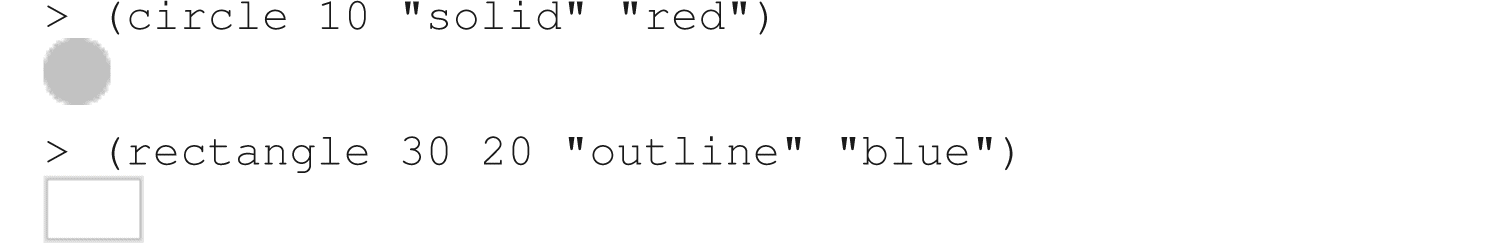
\includegraphics[width=0.85\textwidth]{images/00008.png}
\end{center}

当表达式的求值结果是一张图像时，DrRacket 会直接将其绘制在交互区中。而在程序内部，BSL 将图像视作与数字同等地位的数据。特别地，BSL 拥有用于组合图像的原语操作，正如用加号合并数字、用 \code{string-append} 拼接字符串一样自然：

\begin{center}
  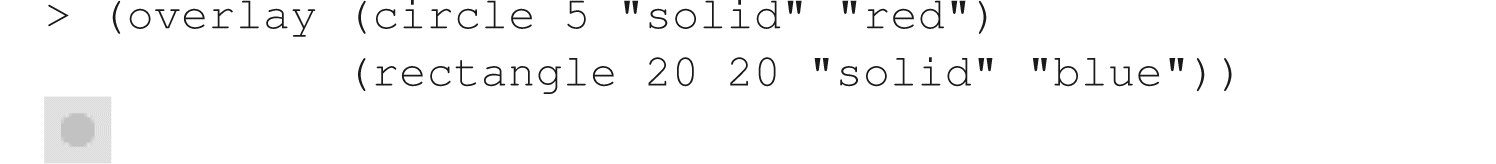
\includegraphics[width=0.85\textwidth]{images/00009.png}
\end{center}

如果将这两个图像按照相反的顺序叠放（将大正方形放在上面），则会得到一个纯蓝色的方块：

\begin{center}
  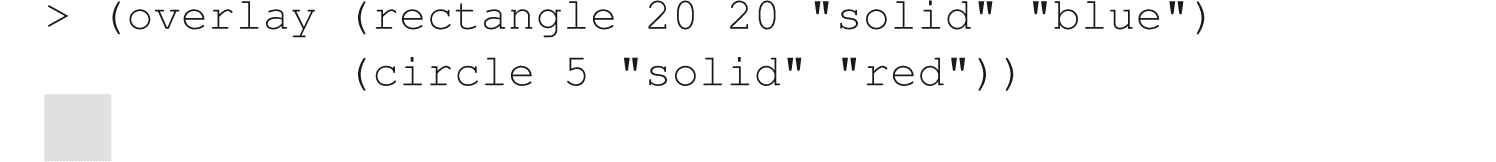
\includegraphics[width=0.85\textwidth]{images/00010.png}
\end{center}

停下来，思考一下为什么最后一个操作会盖住圆盘。

正如你所见，\code{overlay}（重叠）在感觉上比 \code{+} 更接近 \code{string-append}，但它确实是在“相加”图像，正如字符串拼接相加文本、加法操作相加数值一样。以下是关于这一思想的另一个例证：

\begin{replbox}
> (image-width (square 10 "solid" "red"))
10
> (image-width
    (overlay (rectangle 20 20 "solid" "blue")
             (circle 5 "solid" "red")))
20
\end{replbox}

上述与 DrRacket 的交互根本没有绘制任何画面，它们实际上只是在精确度量组合图像的宽度。

最后两个关键操作是 \code{empty-scene}（空场景）与 \code{place-image}（放置图像）。前者用于创建一个被称为\term{场景}（scene）的特殊矩形画布；后者则负责将指定图像精确放置到该场景中：

\begin{lstlisting}[language=BSL]
(place-image (circle 5 "solid" "green")
             50 80
             (empty-scene 100 100))
\end{lstlisting}

你将获得如下画面：

\begin{center}
  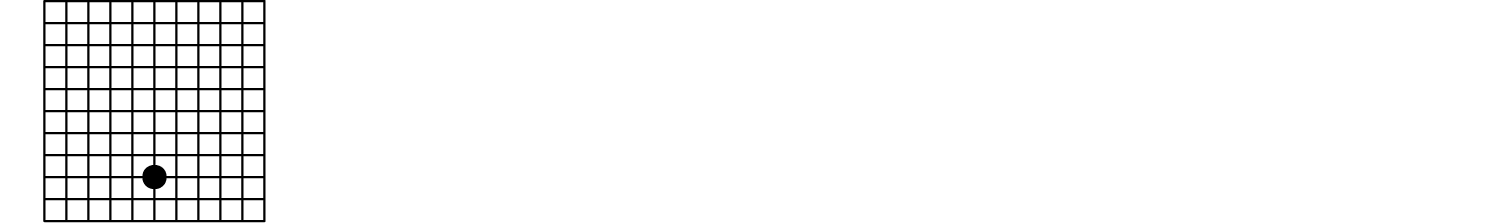
\includegraphics[width=0.35\textwidth]{images/00013.png}
\end{center}

\begin{notebox}[坐标系说明]
生成的真实场景中并没有参考网格线。我们在场景上叠加了坐标网格，以便你能清晰看到绿色圆点具体落在了何处。
\end{notebox}

从这幅图中可以看出，场景的坐标原点 \code{(0,0)} 位于窗口的\textbf{左上角}。与传统的笛卡尔数学坐标系不同，计算机屏幕上的 $y$ 坐标是\textbf{向下}递增的，而非向上。除此之外，画面完全符合预期：在宽 100、高 100 的空白矩形场景中，坐标 \code{(50, 80)} 处清晰地呈现着一个实心绿色圆盘。

让我们再次总结核心心智模型：所谓编程，就是书写清晰的算术表达式，但你的视野绝不再局限于单调的数字。在 BSL 中，算术是囊括了数字、字符串、布尔值乃至丰富图像的宏大算术体系。而计算，依然意味着求出表达式的最终值——只不过这个值可以是一个数字、一段文本、一个真假布尔值，或者一幅绚丽的图像。

现在，你已经彻底做好准备，编写能让小火箭在星空中飞翔的动态程序了！


% ------------------------------------------------------------------------------
\section{输入与输出}
\label{sec:prologue:inputs_output}
% ------------------------------------------------------------------------------

到目前为止，你所写的程序其实还相当局限。写下一行或几行表达式，点击“Run”，看到一些结果；如果再次点击“Run”，看到的依然是分毫不差的相同结果。事实上，无论你点击多少次“Run”，结果永远固定不变。简而言之，你的程序目前不过就像一台功能高级的掌上计算器，只是 DrRacket 能够计算包括图像在内的各种数据而已。

这既是一个好消息，也是一个坏消息。好消息在于：编程与计算本来就应当是计算器运算的自然推广。坏消息在于：编写软件的真正目的，在于用一套相同的计算逻辑去处理海量各异的数据，并动态产生形形色色的不同结果（而且计算速度应当远超人类手工）。也就是说，在掌握真正的编程之道前，我们还需要掌握更强大的工具。不过完全不必担心：凭借你对数字、字符串、布尔值与图像算术的扎实理解，你距离编写一个能够生成连续动画甚至电影的大作仅有一步之遥，绝非只是输出一句幼稚的“hello world”。这正是我们接下来的目标。

动画或电影本质上就是以极高频率按顺序快速连续放映的一组画面序列。如果你的代数老师当年知晓我们在上一节看到的“图像算术”，你们当年在代数课堂上完全可以制作精彩的电影，而不是计算枯燥的数字序列。不妨重温中学代数中常见的这种表格：

\begin{center}
\small
\setlength{\tabcolsep}{3.5pt}
\begin{tabular}{lcccccccccc}
  $x =$ & 1 & 2 & 3 & 4 & 5 & 6 & 7 & 8 & 9 & 10 \\
  \hline
  $y =$ & 1 & 4 & 9 & 16 & 25 & 36 & 49 & 64 & 81 & ?
\end{tabular}
\end{center}

代数老师通常会要求你在表格空白处填空，即用正确的数字替换问号“\code{?}”。

事实证明，制作动画丝毫不比完成这样一张数字表格复杂。事实上，动画的本质完全基于这种对照表格：

\begin{center}
  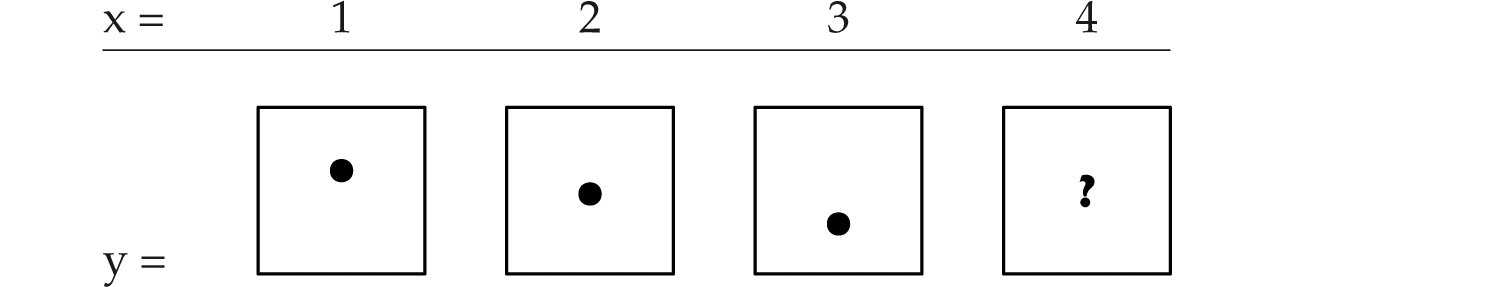
\includegraphics[width=0.85\textwidth]{images/00015.png}
\end{center}

具体来说，老师在这里会要求你画出第四个、第五个乃至第 1273 个画面，因为电影就是大量连续画面的集合（通常每秒需要 24 到 30 幅画面）。要制作一分钟的动画，大约需要 1200 到 1800 幅画面。

你也许还记得，代数老师不仅要求你计算序列中的第四或第五个数值，还会要求你写出一个通用的数学表达式，能够根据任意给定的输入 $x$ 计算出对应的输出 $y$。在纯数字的例子中，老师期待看到的答案通常是这样的：

\[
  y = x \cdot x
\]

只要将 1、2、3 等代入 $x$，便能依次求出对应的 $y$ 为 1、4、9 等——正如表格所记录的那样。而对于图像序列，你可以将其表述为：
\begin{quote}
$y =$ 包含一个距离场景顶部 $x^2$ 像素的圆点的画面。
\end{quote}
核心要点在于：这些能够统摄全局的规律单行式，已经不再是静态的表达式，而是\term{函数}（functions）！

乍看之下，函数长得很像表达式：左边总是一个 $y$，中间是一个等号，右边是一个算式。然而，它们绝非单纯的表达式。学校里关于函数的传统记法往往极具误导性。因此在 DrRacket 中，我们采用更清晰明确的记法来书写函数：
\begin{lstlisting}[language=BSL]
(define (y x) (* x x))
\end{lstlisting}

这里的关键字 \code{define} 表示“将 \code{y} 定义为一个函数”，它与表达式类似，用于计算出一个值。然而，函数的值取决于被称为\term{输入}（input）的动态值，我们通过 \code{(y x)} 来声明这一点。由于在定义函数时尚不知道具体输入是多少，我们使用一个名字来代表未知的输入。遵循代数传统，我们在这里用 \code{x} 代表未知的输入；不过很快，我们就会使用更具描述性的各种有意义的名称。

第二部分表明，你必须为 \code{x} 提供一个具体的数值，才能计算出 \code{y} 的具体结果。当你提供该数值时，DrRacket 会将该数值代入函数关联的主体表达式中。在这里主体表达式是 \code{(* x x)}。一旦 \code{x} 被具体数值（例如 1）替换，DrRacket 就能算出表达式的结果，该结果被称为函数的\term{输出}（output）。

\begin{notebox}[数学记法对比]
数学中常将 $y(1)$ 称为一次“函数应用”（function application），只是很多老师在课堂上忽略了向大家强调这个术语。
\end{notebox}

点击“Run”，你会发现什么动静都没有。交互区既没有打印任何结果，DrRacket 界面其他地方似乎也没有任何变化。你可能会觉得自己仿佛什么都没做成。但实际上你完成了一件大事：你成功定义了一个函数，并向 DrRacket 正式通告了它的存在！DrRacket 现在已经完全准备好供你随时调用该函数了。在交互区的提示符后输入：
\begin{replbox}
> (y 1)
1
\end{replbox}
这里的 \code{(y 1)} 在 DrRacket 中被称为一次\term{函数应用}（function application）或函数调用。再尝试：
\begin{replbox}
> (y 2)
4
\end{replbox}
便能看到 4 跃然眼前。当然，你也可以把这些测试调用全部写在定义区中，然后点击“Run”：
\begin{lstlisting}[language=BSL]
(define (y x) (* x x))
(y 1)
(y 2)
(y 3)
(y 4)
(y 5)
\end{lstlisting}
DrRacket 会在交互区依次输出：\code{1 4 9 16 25}，精准对应表格中的全部数值。现在，试着算出刚才表格中遗漏的第 1273 个数值吧！

这一切对于你而言意味着：函数提供了一种极其经济而强大的机制，只需一个统一的表达式，便能计算出无穷无尽的有趣结果。事实上，\textbf{程序本质上就是函数}；一旦透彻理解了函数，你就掌握了关于编程几乎所有核心奥秘的大门钥匙。鉴于其至高无上的地位，让我们系统梳理迄今为止关于函数的全部知识：
\begin{itemize}
  \item 首先，\code{(define (FunctionName InputName) BodyExpression)} 是\textbf{函数定义}。你能通过开头的 \code{define} 关键字瞬间认出它。它本质上由三部分构成：两个名称和一个表达式。第一个名称是函数本身的名称（\code{FunctionName}），你需要它来随心所欲地多次调用该函数；第二个名称被称为\term{形参}（parameter，即 \code{InputName}），代表在具体调用发生前未知的输入数据；最后的主体表达式（\code{BodyExpression}，称为\term{函数体}）负责根据具体输入计算出函数的输出。
  
  \item 其次，\code{(FunctionName ArgumentExpression)} 是\textbf{函数应用}（函数调用）。第一项指明你想要调用哪个函数；第二项则是作为输入传给该函数的具体实参表达式（\code{ArgumentExpression}）。如果是读桌面软件的说明书，可能会说该表达式“启动”了名为 \code{FunctionName} 的“应用程序”，并将 \code{ArgumentExpression} 作为输入传递给它。与所有表达式一样，实参可以是一个纯数据常量，也可以是一个深度嵌套的复杂子表达式。
\end{itemize}

函数的输入绝不仅限于数字，它们的输出也可以是任何丰富的数据形态。我们接下来的目标是创建一个能够模拟第二个表格（小圆点逐帧降落的场景图像序列）的函数，正如刚才的函数模拟了纯数字表格一样。由于利用表达式生成图像在中学阶段并未普及，让我们从最直观的步骤开始操练。还记得上一节末尾提到的 \code{empty-scene} 吗？在交互区输入：

\begin{center}
  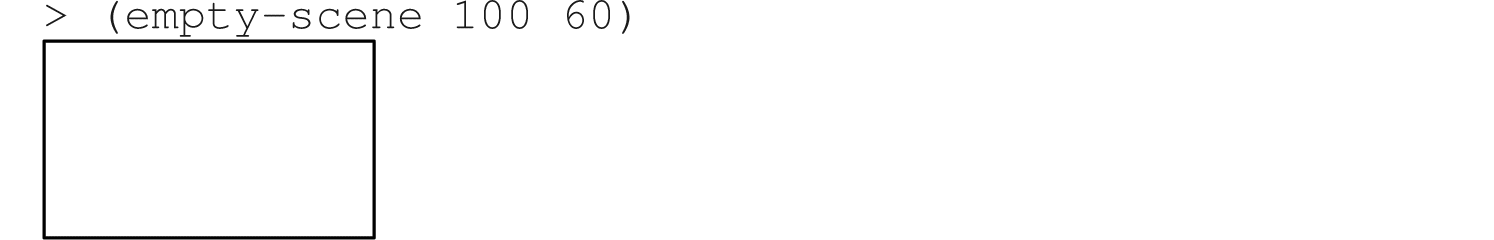
\includegraphics[width=0.85\textwidth]{images/00017.png}
\end{center}

DrRacket 会立即生成一个空白的矩形场景。我们可以利用 \code{place-image} 向该场景中置入图像：

\begin{center}
  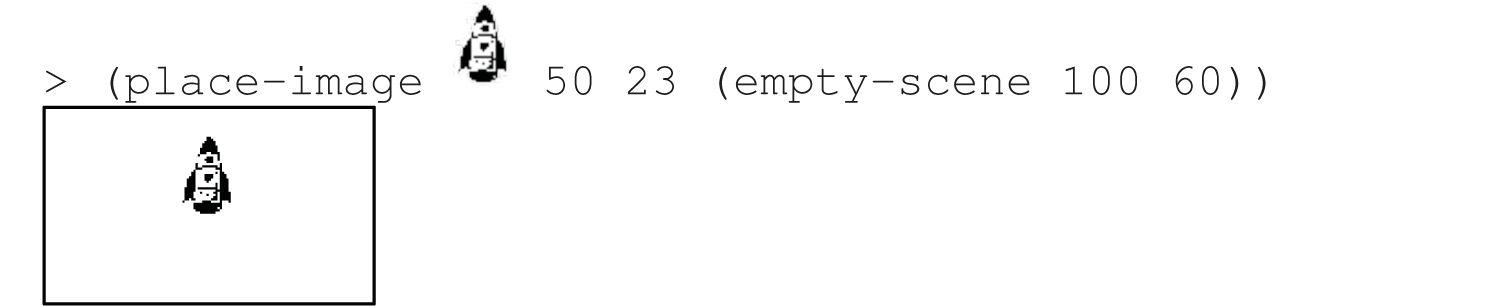
\includegraphics[width=0.85\textwidth]{images/00018.jpeg}
\end{center}

不妨把小火箭想象成数学课表格中的小圆点，唯一的不同在于：小火箭比单调的圆点有趣生动得多！

接下来，我们应该让小火箭平稳降落，正如表格中小圆点不断向下位移一样。从上一节我们已经知道，只需在调用 \code{place-image} 时递增传入的 $y$ 坐标数值，便能轻松实现这一效果：

\begin{center}
  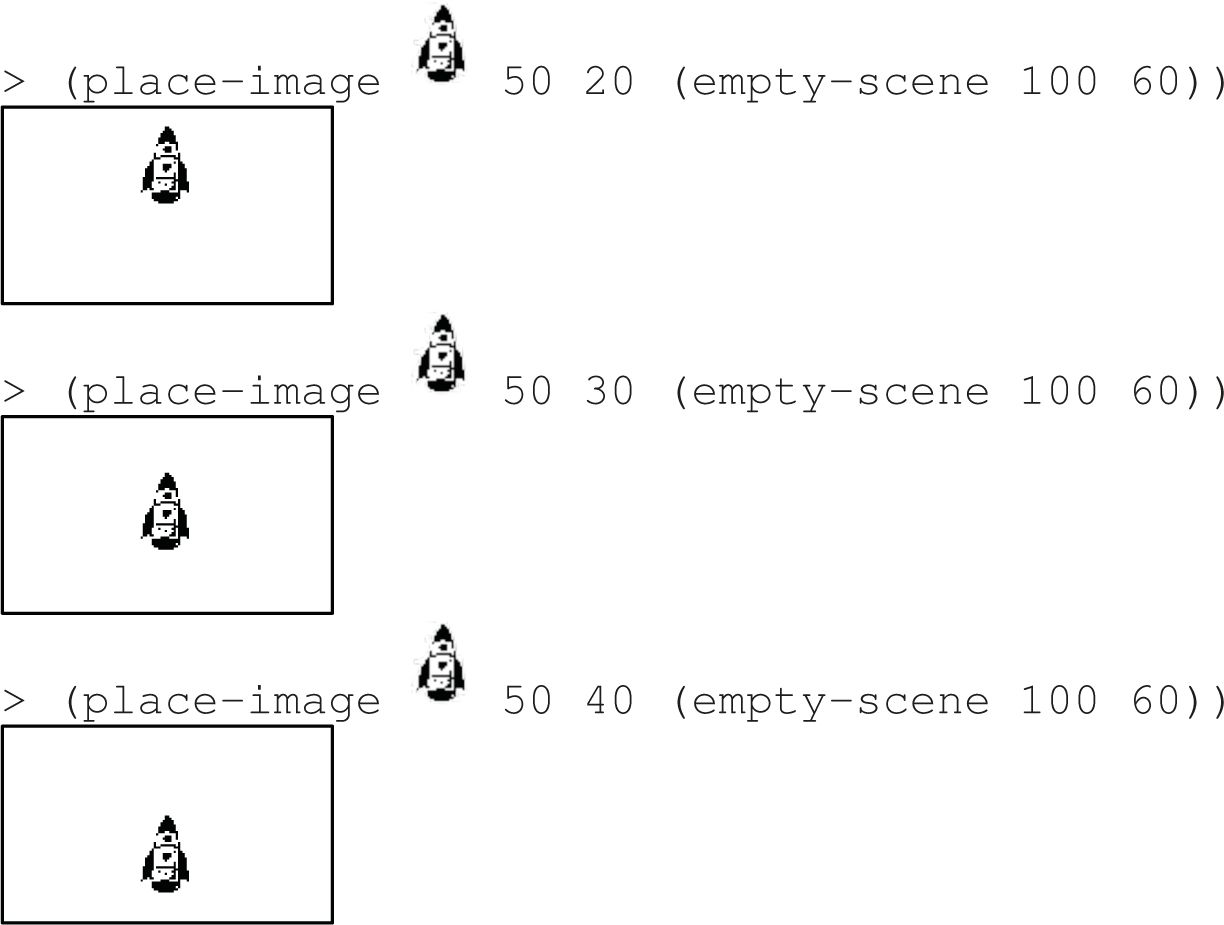
\includegraphics[width=0.75\textwidth]{images/00019.jpeg}
\end{center}

现在剩下的唯一任务，就是如何轻松大量地生成这类连续场景，并以极快的速度依次将它们连续播放出来。

第一个目标当然可以通过定义一个函数轻松达成，参见图~\ref{fig:rocket_v1}。没错，这是一个货真价实的函数定义！我们没有使用晦涩单调的字母 \code{y}，而是为其赋予了一个顾名思义的名称 \code{picture-of-rocket}（火箭画面），一眼就能看出该函数的输出是一个包含火箭的场景画面。在参数命名上，我们没有使用抽象的字母 \code{x}，而是采用了 \code{height}（高度），这直观表明它是一个数字，且明确告诉函数应当将火箭放置在场景中的哪个高度位置。函数体表达式与我们刚才反复操练的表达式完全相同，唯一的不同在于用形参 \code{height} 替换了具体的硬编码数字。现在，我们可以利用这一个函数轻松创建任意高度的画面：
\begin{lstlisting}[language=BSL]
(picture-of-rocket 0)
(picture-of-rocket 10)
(picture-of-rocket 20)
(picture-of-rocket 30)
\end{lstlisting}

\begin{figure}[htbp]
  \centering
\begin{stepperbox}[unbreakable]
\begin{Verbatim}[commandchars=\\\{\}, fontsize=\scriptsize]
(define (picture-of-rocket height)
  (place-image \inlinesprite[1.4em]{images/sprites/rocket.png} 50 height (empty-scene 100 60)))
\end{Verbatim}
\end{stepperbox}
  \caption{火箭降落程序（版本 1）}
  \label{fig:rocket_v1}
\end{figure}

在定义区或交互区中输入上述调用；两者都能立刻生成完全符合预期的连续画面。

\begin{notebox}[BSL 标识符命名规范]
在 BSL 中，你可以使用各种丰富的字符来为函数或变量命名，包括连字符“\code{-}”和点号“\code{.}”，这让名称具备极佳的自解释性。
\end{notebox}

要达成第二个目标（快速连续播放生成动态电影），我们需要从 \code{2htdp/universe} 教学包中请出一位关键原语：\term{animate}（动画控制器）。点击“Run”，在交互区中输入以下神奇的表达式：
\begin{replbox}
> (animate picture-of-rocket)
\end{replbox}

\begin{notebox}[引入动画教学包]
别忘了在定义区最上方添加 \code{(require 2htdp/universe)}，以导入宇宙/世界程序库。
\end{notebox}

停下来，请特别注意：\textbf{这里的参数本身是一个函数名}！目前不必对将函数作为参数感到深奥或顾虑；它在 \code{animate} 中工作得极其出色，不过初学阶段暂且不要尝试自己编写像 \code{animate} 这样以函数作为参数的高阶函数。

当你按下回车键的一刹那，DrRacket 会立刻对该表达式求值；但它并不会在交互区输出任何普通的静态文本，甚至提示符也不会立刻出现。相反，它会单独弹出一个崭新的独立动画窗口（画布），并启动一个每秒钟跳动 28 次的高精度时钟！每当时钟滴答跳动一次，DrRacket 就会自动调用 \code{picture-of-rocket} 函数，并将“自启动以来所流逝的时钟滴答总数”（0、1、2、3……）作为实参传入。这些函数调用所生成的场景画面被源源不断地刷新绘制在画布上，从而在视网膜上形成了流畅逼真的动态火箭降落动画！动画会一直持续运行，直到你手动关闭该窗口为止；此时 \code{animate} 会在交互区返回动画总共经历的时钟滴答数。

这个动画背后的本质运行机制是什么？简短的解释是：\code{animate} 将其操作数（即传入的函数）依次应用于数字 0、1、2、3……并实时呈现生成的连续画面。详细的机制如下：
\begin{itemize}
  \item \code{animate} 启动一个独立时钟，并对滴答步数进行自增计数；
  \item 时钟以每秒 28 次的恒定频率跳动；
  \item 每次时钟滴答，\code{animate} 都会以当前时钟计数为参数调用 \code{picture-of-rocket} 函数；
  \item 该次调用所返回的全新场景被立即投射显示在动画画布上。
\end{itemize}

这意味着小火箭首先出现在高度 0 处，接着是高度 1、高度 2……这完美解释了为什么小火箭会从画布顶部平稳地降落到底部。也就是说，我们仅仅用了区区三行代码的微型程序，就在短短 3.5 秒内自动生成了约 100 张连续画面，并通过超高速放映创造出逼真的火箭降落视觉奇观！

\begin{notebox}[关于 animate 的原理]
在全书后半部分的练习 298 中，我们将带领大家亲手从底层设计实现出属于自己的 \code{animate} 核心引擎。
\end{notebox}

回顾本节，你学到了至关重要的核心知识：函数之所以威力无穷，是因为它们能够在极短时间内批量自动化处理海量数据。你可以手动在少数几个精心挑选的典型输入上测试函数，以确保它产出完全正确的预期结果，这被称为\term{测试函数}（testing a function）。或者，DrRacket 可以在各类外部库的配合下，自动在海量数据流上连续调用该函数，这被称为\term{运行函数}（running a function）。自然，DrRacket 也能在用户敲击键盘或滑动鼠标时自动触发函数的调用。究竟是什么事件触发了函数的执行并不重要，但请永远牢记：\textbf{（简单）程序在本质上就是函数}。


% ------------------------------------------------------------------------------
\section{多样化的计算方式}
\label{sec:prologue:many_ways}
% ------------------------------------------------------------------------------

当你运行 \code{(animate picture-of-rocket)} 时，小火箭最终会直直地穿透场景底部并沉入地底深渊消失不见。这显然违背常识。在老科幻电影中，火箭绝不会无休止地遁入地心，而是会优雅地用尾部平稳着陆在地面上，动画也应当在着陆的瞬间圆满落幕。

这一需求表明：\textbf{计算应当根据现实情境的不同，走向截然不同的逻辑分支}。在我们的案例中，当火箭尚在空中飞行时，\code{picture-of-rocket} 应当按原样绘制动态下落；然而一旦火箭的尾部触及画布底部，程序就应当立即阻止火箭继续下潜。

从某种意义上说，这种思想对你而言毫不陌生。甚至连中学数学老师在定义函数时，也会根据不同情形进行条件分流：

\[
  \mathrm{sign}(x) = \begin{cases}
    +1 & \text{if } x > 0 \\
    \phantom{+}0 & \text{if } x = 0 \\
    -1 & \text{if } x < 0
  \end{cases}
\]

这个符号函数 $\mathrm{sign}(x)$ 明确区分了三种输入情境：大于 0 的正数、等于 0 的数值以及小于 0 的负数。根据输入落入的区间，函数分别返回 $+1$、$0$ 或 $-1$。

在 DrRacket 中，你可以借助\term{条件表达式}（conditional expression，简称 \code{cond}）毫无困难地将这种分段函数原汁原味地翻译为代码：

\begin{lstlisting}[language=BSL]
(define (sign x)
  (cond
    [(> x 0) 1]
    [(= x 0) 0]
    [(< x 0) -1]))
\end{lstlisting}

点击“Run”后，你就可以像测试任何普通函数一样在交互区与 \code{sign} 进行交互：
\begin{replbox}
> (sign 10)
1
> (sign -5)
-1
> (sign 0)
0
\end{replbox}

\begin{notebox}[在 DrRacket 中开启新标签页]
可以在 DrRacket 中点击“File”菜单选择“New Tab”（新建标签页），开启一个干干净净的全新工作区进行实验。
\end{notebox}

在语法结构上，条件表达式的一般形式如下：
\begin{lstlisting}[language=BSL]
(cond
  [ConditionExpression1 ResultExpression1]
  [ConditionExpression2 ResultExpression2]
  ...
  [ConditionExpressionN ResultExpressionN])
\end{lstlisting}

\begin{notebox}[探索代数单步求值器]
现在是体验 DrRacket 中“Step”（单步求值器）神奇魅力的绝佳时机！在定义区添加 \code{(sign -5)}，然后点击工具栏右上角的“Step”按钮。在弹出的单步求值器窗口中，点击左右箭头，亲眼观察表达式一步一步被替代求值的全过程！
\end{notebox}

也就是说，一个条件表达式由若干行条件分支（clauses）构成。每一行包含两个子表达式：位于左侧的通常称为\term{条件}（condition，有时也称问题/断言），位于右侧的称为\term{结果}（result，有时也称答案）。当 DrRacket 对一个 \code{cond} 表达式进行求值时，它首先计算第一个条件表达式 \code{ConditionExpression1}：
\begin{itemize}
  \item 如果求值结果为 \code{\#true}，DrRacket 会立刻将整个 \code{cond} 表达式替换为对应的 \code{ResultExpression1}，对其求值并将该值作为整个条件表达式的最终结果；
  \item 如果求值结果为 \code{\#false}，DrRacket 会彻底忽略该分支，转而对下一行重复相同的判定；
  \item 如果所有行的条件表达式求值结果均为 \code{\#false}，DrRacket 会直接报错，指出没有满足任何条件分支。
\end{itemize}

掌握了这一利器，我们现在便能从容改变火箭模拟动画的运转轨迹了。目标是：绝不让小火箭下降到 100 $\times$ 60 场景的地面以下。由于 \code{picture-of-rocket} 函数接收一个代表火箭在场景中所处高度的数字实参，只需引入一个简单的测试，将传入的当前高度与最大极限高度进行比对即可。

参见图~\ref{fig:rocket_v2} 中的修正后函数定义。为了区分两个版本，我们在新定义中使用名称 \code{picture-of-rocket.v2}。使用不同的函数名还允许我们在交互区同时调用两个版本，并直观对比它们的行为差异。以下是最初版本 1 的运行效果：

\begin{center}
  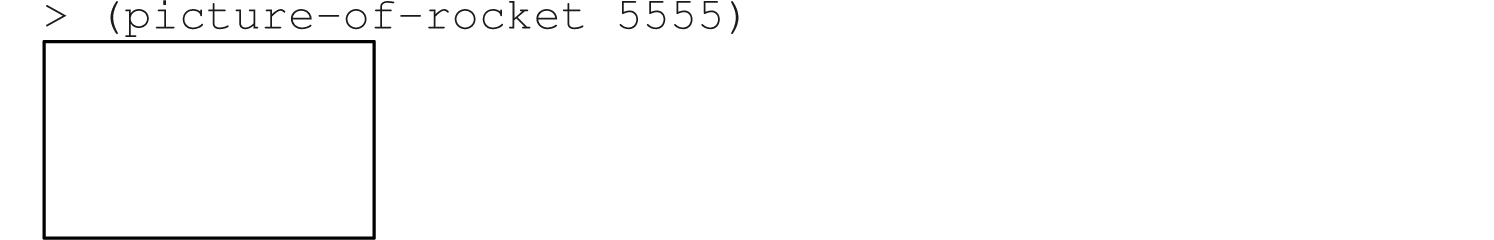
\includegraphics[width=0.85\textwidth]{images/00023.png}
\end{center}

\begin{figure}[htbp]
  \centering
\begin{stepperbox}[unbreakable]
\begin{Verbatim}[commandchars=\\\{\}, fontsize=\footnotesize]
(define (picture-of-rocket.v2 height)
  (cond
    [(<= height 60)
     (place-image \inlinesprite[1.4em]{images/sprites/rocket.png} 50 height
                  (empty-scene 100 60))]
    [(> height 60)
     (place-image \inlinesprite[1.4em]{images/sprites/rocket.png} 50 60
                  (empty-scene 100 60))]))
\end{Verbatim}
\end{stepperbox}
  \caption{火箭降落程序（版本 2）}
  \label{fig:rocket_v2}
\end{figure}

以下是全新版本 2 的运行效果：

\begin{center}
  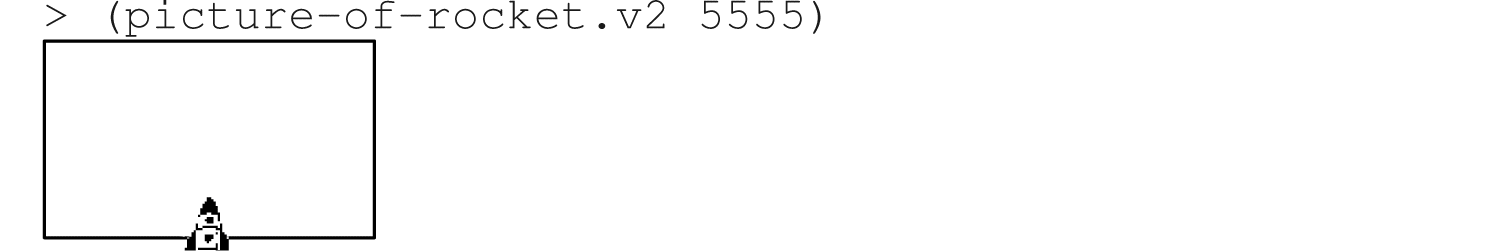
\includegraphics[width=0.85\textwidth]{images/00025.png}
\end{center}

无论你传递给 \code{picture-of-rocket.v2} 多大的数字，只要它超过了 60，得到的永远是同一幅固定在底部的画面。特别地，当你在交互区执行：
\begin{replbox}
> (animate picture-of-rocket.v2)
\end{replbox}
小火箭在下降后，会在正好陷进地面一半的位置赫然停住！

\begin{notebox}[思考提问]
停下来想一想！这真的是我们期望看到的完美着陆吗？
\end{notebox}

让火箭半截身子陷进泥土里显然很不雅观。不过，你完全清楚如何修复这一瑕疵。正如你所见，BSL 精通图像算术。当 \code{place-image} 将一幅图像绘制到场景中时，它默认将该图像的\textbf{几何中心点}作为对齐锚点，尽管图像本身拥有真实的物理宽度与高度。你一定还记得，我们可以使用 \code{image-height} 随时测量出图像的准确高度。这个操作在这里派上了大用场，因为我们真正希望的是：让火箭平稳飞行，直到其\textbf{底面触及地面}的那一刻停止。

把各方线索串联起来，你就能通过算术推导出：

\begin{stepperbox}
\begin{Verbatim}[commandchars=\\\{\}, fontsize=\footnotesize]
(- 60 (/ (image-height \inlinesprite[1.4em]{images/sprites/rocket.png}) 2))
\end{Verbatim}
\end{stepperbox}

正是火箭停止下降时其中心点应当停留的准确位置！你可以通过直接修改程序来验证这一推断，也可以在交互区利用图像算术即时验证。

以下是初步的尝试：

\begin{stepperbox}
\begin{Verbatim}[commandchars=\\\{\}, fontsize=\footnotesize]
(place-image \inlinesprite[1.4em]{images/sprites/rocket.png} 50 (- 60 (image-height \inlinesprite[1.4em]{images/sprites/rocket.png}))
             (empty-scene 100 60))
\end{Verbatim}
\end{stepperbox}

现在，把上面调用中的第三个实参替换为：

\begin{stepperbox}
\begin{Verbatim}[commandchars=\\\{\}, fontsize=\footnotesize]
(- 60 (/ (image-height \inlinesprite[1.4em]{images/sprites/rocket.png}) 2))
\end{Verbatim}
\end{stepperbox}

\begin{notebox}[动手实验]
停下来，在 DrRacket 中亲身运行对比这两个调用。你更钟意哪一个视觉呈现？
\end{notebox}

沿着这一思路深入思考与反复验证，最终你就会自然而然地写出如图~\ref{fig:rocket_v3} 所示的优雅程序。给定一个代表火箭飞行高度的数字，它首先检测火箭的底端是否尚在地表之上。如果是，它像以前一样将火箭绘制在当前飞行高度；如果不是，它将火箭放置在底端正好贴合地面的精确几何位置！

\begin{figure}[htbp]
  \centering
\begin{stepperbox}[unbreakable]
\begin{Verbatim}[commandchars=\\\{\}, fontsize=\scriptsize]
(define (picture-of-rocket.v3 height)
  (cond
    [(<= height (- 60 (/ (image-height \inlinesprite[1.4em]{images/sprites/rocket.png}) 2)))
     (place-image \inlinesprite[1.4em]{images/sprites/rocket.png} 50 height
                  (empty-scene 100 60))]
    [(> height (- 60 (/ (image-height \inlinesprite[1.4em]{images/sprites/rocket.png}) 2)))
     (place-image \inlinesprite[1.4em]{images/sprites/rocket.png} 50 (- 60 (/ (image-height \inlinesprite[1.4em]{images/sprites/rocket.png}) 2))
                  (empty-scene 100 60))]))
\end{Verbatim}
\end{stepperbox}
  \caption{火箭降落程序（版本 3）}
  \label{fig:rocket_v3}
\end{figure}


% ------------------------------------------------------------------------------
\section{一个程序，多个定义}
\label{sec:prologue:one_program_many_definitions}
% ------------------------------------------------------------------------------

现在设想你的朋友们观赏了你的火箭降落动画，但他们觉得默认的画布尺寸太局促了，希望能将其扩展为 200 $\times$ 400 的宽阔大场景。面对这个看似简单的需求变更，你不得不痛苦地在程序中的五个不同地方把 100 逐一替换为 400，在另外两个地方把 60 逐一替换为 200——更不必说代码中那些代表“画布水平中线”的数字 50 了。

\begin{notebox}[动手体验硬编码之痛]
在继续阅读前，请务必停下来动手尝试手动修改这些数字！亲身体验一下在区区五行代码的程序中完成这一改动是多么容易漏改改错。在阅读后续内容时，请时刻牢记：现实工业界中的软件规模往往长达 50,000 行、500,000 行乃至 5,000,000 行以上的庞大代码库！
\end{notebox}

在一个设计优良的理想程序中，一个微小的需求调整（比如修改画布尺寸），应当仅仅需要对应一处微小的代码修改。在 BSL 中实现这一优雅解耦的利器依然是 \code{define}。除了定义函数，\code{define} 还能用于定义\term{常量}（constants），即将一个有意义的名字与一个固定常量值绑定在一起。常量定义的一般形式极为简洁：
\begin{lstlisting}[language=BSL]
(define Name Expression)
\end{lstlisting}

举例来说，如果在程序中写下：
\begin{lstlisting}[language=BSL]
(define HEIGHT 60)
\end{lstlisting}
你就是在向 DrRacket 声明：全局名称 \code{HEIGHT} 始终代表数字 60。这种定义的语义完全符合常识：每当 DrRacket 在后续计算中遇到标识符 \code{HEIGHT} 时，它都会自动用 60 替换之。

现在请仔细审视遵照这一设计原则重构出的图~\ref{fig:rocket_v4}。它落实了这一改动，并且为小火箭图像也赋予了一个直观的名字。将该程序复制到 DrRacket 中，点击“Run”后在交互区执行：
\begin{replbox}
> (animate picture-of-rocket.v4)
\end{replbox}
确认该程序的功能与之前的版本 3 完全一致。

\begin{figure}[htbp]
  \centering
\begin{stepperbox}[unbreakable]
\begin{Verbatim}[commandchars=\\\{\}, fontsize=\scriptsize]
(define (picture-of-rocket.v4 h)
  (cond
    [(<= h (- HEIGHT (/ (image-height ROCKET) 2)))
     (place-image ROCKET 50 h (empty-scene WIDTH HEIGHT))]
    [(> h (- HEIGHT (/ (image-height ROCKET) 2)))
     (place-image ROCKET
                  50 (- HEIGHT (/ (image-height ROCKET) 2))
                  (empty-scene WIDTH HEIGHT))]))

(define WIDTH 100)
(define HEIGHT 60)
(define ROCKET \inlinesprite[1.4em]{images/sprites/rocket.png})
\end{Verbatim}
\end{stepperbox}
  \caption{火箭降落程序（版本 4）}
  \label{fig:rocket_v4}
\end{figure}

图~\ref{fig:rocket_v4} 中的程序共包含四个顶层定义：一个函数定义与三个常量定义。数字 100 与 60 在整个程序中各自仅出现了一次——分别作为 \code{WIDTH} 与 \code{HEIGHT} 的值。你可能还注意到，我们将函数形参从 \code{height} 缩写为了 \code{h}。严格来说这一修改并非必需，因为 DrRacket 能够严格区分小写的 \code{height} 与大写的常量 \code{HEIGHT}，但为了避免读者在视觉上产生混淆，我们特意做了区分。

当 DrRacket 执行 \code{(animate picture-of-rocket.v4)} 时，每当它在计算中遇到这些名字，都会自动将 \code{HEIGHT} 替换为 60、\code{WIDTH} 替换为 100、\code{ROCKET} 替换为具体的火箭图像。为了亲身体验真正程序员的高光时刻，请将 \code{HEIGHT} 后面的 60 改为 400，然后轻点“Run”。你将瞬间看到小火箭在宽 100、高 400 的宏大高空场景中优雅降落！\textbf{仅仅改动一个数字，全局牵一发而动全身}。

在现代软件工程术语中，你刚刚亲身经历了人生的第一次\term{代码重构}（program refactoring）。每当你为了让程序更好地适应未来潜在的需求变更而重新梳理和优化其架构时，你都在对程序进行重构。把这个词骄傲地写进你的简历吧，它听起来专业干练，你未来的雇主一定会乐于看到这样的工程素养。然而，任何一个真正优秀的程序员都绝不可能容忍在同一个程序中将完全相同的子表达式重复书写三次：
\begin{lstlisting}[language=BSL]
(- HEIGHT (/ (image-height ROCKET) 2))
\end{lstlisting}

每当你的同事或未来的你自己阅读这段代码时，都必须费神去重新推导该表达式究竟在算什么（即场景顶部到落地火箭中心点的距离）。每当 DrRacket 计算该表达式时，它都必须死板地重复三步计算：(1) 测量图像高度；(2) 除以 2；(3) 从 \code{HEIGHT} 中减去该值。而且每一次算出的都是完全相同的定值！

这一观察强烈呼唤我们引入一个新的常量定义：
\begin{lstlisting}[language=BSL]
(define ROCKET-CENTER-TO-TOP
  (- HEIGHT (/ (image-height ROCKET) 2)))
\end{lstlisting}

现在，在程序的其余部分中，用名字 \code{ROCKET-CENTER-TO-TOP} 彻底替换掉那长长的一串表达式。你可能会琢磨：这个新常量定义到底应该放在 \code{HEIGHT} 之上还是之下？更普适地讲，程序中定义的排列顺序是否至关重要？答案是：\textbf{对于常量定义，先后顺序至关重要；而对于函数定义，顺序则完全无关紧要}。一旦 DrRacket 读到一个常量定义，它会立即对等号右边的表达式求值，并立即将名称与该结果值永久绑定。例如：
\begin{lstlisting}[language=BSL]
(define HEIGHT (* 2 CENTER))
(define CENTER 100)
\end{lstlisting}
会导致 DrRacket 在执行第一行时严厉报错：“\code{CENTER} 在定义之前就被使用了”。相反：
\begin{lstlisting}[language=BSL]
(define CENTER 100)
(define HEIGHT (* 2 CENTER))
\end{lstlisting}
则完全顺畅运行。首先，DrRacket 将 \code{CENTER} 绑定为 100；其次，对 \code{(* 2 CENTER)} 求值得出 200；最后，将 200 绑定至 \code{HEIGHT}。

尽管常量之间的定义先后顺序不可颠倒，但常量定义相对于函数定义的相对位置却完全自由。事实上，如果你的程序由许多函数定义组成，函数彼此之间的摆放顺序也完全任意；但最佳的工程实践是：\textbf{首先集中声明所有全局常量定义，随后按照重要程度降序排列各个函数定义}。当你日后开始独立编写包含数十个定义的复杂大型项目时，你就会深刻体会到这种清晰组织纪律的无穷益处。

\begin{notebox}[关于代码注释]
程序中还可以包含以分号（\code{;}）开头的单行注释。尽管 DrRacket 运行时会彻底忽略所有注释，但阅读代码的人类绝不应忽视它们。注释是程序的创作者与未来的维护者之间跨越时空的“秘密沟通热线”，用于传递代码本身难以自述的架构意图。
\end{notebox}

一旦清除了所有重复冗余的表达式，我们便收获了如图~\ref{fig:rocket_v5} 所示的纯净版本。它由一个主函数定义与五个精心提炼的常量定义组成。除了火箭落地中心点位置外，这些常量还将火箭图像资源本身以及空白背景场景的构建完全抽取成了独立组件。

\begin{figure}[htbp]
  \centering
\begin{stepperbox}[unbreakable]
\begin{Verbatim}[commandchars=\\\{\}, fontsize=\scriptsize]
; constants
(define WIDTH  100)
(define HEIGHT  60)
(define MTSCN  (empty-scene WIDTH HEIGHT))
(define ROCKET \inlinesprite[1.4em]{images/sprites/rocket.png})
(define ROCKET-CENTER-TO-TOP
  (- HEIGHT (/ (image-height ROCKET) 2)))

; functions
(define (picture-of-rocket.v5 h)
  (cond
    [(<= h ROCKET-CENTER-TO-TOP)
     (place-image ROCKET 50 h MTSCN)]
    [(> h ROCKET-CENTER-TO-TOP)
     (place-image ROCKET 50 ROCKET-CENTER-TO-TOP MTSCN)]))
\end{Verbatim}
\end{stepperbox}
  \caption{火箭降落程序（版本 5）}
  \label{fig:rocket_v5}
\end{figure}

在继续翻页之前，请结合版本 5 深入思考并尝试动手实现以下改进：
\begin{itemize}
  \item 如何修改程序，使其呈现 200 $\times$ 400 的宽阔场景？
  \item 如何修改程序，使其降落的不再是火箭，而是一个绿色的不明飞行物（UFO 飞碟）？绘制飞碟其实极其容易：
\begin{lstlisting}[language=BSL]
(overlay (circle 10 "solid" "green")
         (rectangle 40 4 "solid" "green"))
\end{lstlisting}
  \item 如何修改程序，使太空背景始终呈现出深邃的纯蓝色？
  \item 如何修改程序，让火箭最终停靠在一块比场景底部高出 10 像素的平坦岩石停机坪上？别忘了相应更新背景场景中的地貌绘制！
\end{itemize}

心动不如行动。亲自编写与调试代码是掌握程序设计的唯一康庄大道。别犹豫，现在就打开 DrRacket 大展身手吧！

\paragraph{告别魔法数字（Magic Numbers）}
再次仔细打量 \code{picture-of-rocket.v5}。因为我们消除了所有重复表达式，除却一个数字外，所有的字面数值都从该函数定义中彻底消失了。在专业编程领域，那些散落在代码深处不知其意的裸露数字被称为\term{魔法数字}（magic numbers），没有任何专业工程师会喜欢它们。因为要不了多久，你自己都会忘却这个数字在几何运算中究竟代表什么含义、哪些改动是安全合法的。最稳健的策略始终是用一个有意义的常量定义为其命名。

在这里我们清楚知道：数字 50 代表我们为小火箭选定的水平 $x$ 坐标。尽管单个数字 50 看起来算不上复杂的长算式，但它在本质上也是一个反复出现的重复表达式。因此，我们有充分的理由将 50 从函数体中提炼出来，这个小练习就作为礼物留给你亲手完成吧！


% ------------------------------------------------------------------------------
\section{再添一个定义}
\label{sec:prologue:one_more_definition}
% ------------------------------------------------------------------------------

请回想一下：\code{animate} 传递给其处理函数的实参，本质上是自启动以来\textbf{所经历的时钟滴答总数}！也就是说，传入 \code{picture-of-rocket} 的参数根本不是什么“高度”，而是“\textbf{时间}”。我们之前在所有版本的 \code{picture-of-rocket} 中使用的形参名称其实全都是错误的；我们不应使用代表高度的 \code{h}，而应当使用代表时间的 \code{t}：

\begin{lstlisting}[language=BSL]
(define (picture-of-rocket t)
  (cond
    [(<= t ROCKET-CENTER-TO-TOP)
     (place-image ROCKET 50 t MTSCN)]
    [(> t ROCKET-CENTER-TO-TOP)
     (place-image ROCKET
                  50 ROCKET-CENTER-TO-TOP
                  MTSCN)]))
\end{lstlisting}

而对参数命名的这一微小修正，立刻把程序深层隐藏的一个荒谬漏洞暴露无遗：这个程序竟然把“时间”硬生生当成了“空间距离”来使用！这是多么离谱的设计纰漏啊。

\begin{notebox}[危险预警]
本节需要引入一条基础的初中物理常识。如果你对物理感到头疼，初读时大可放心略过；真正的日常程序设计通常并不需要你通晓物理学知识。
\end{notebox}

即使你从未学过物理，你也必定知晓时间与位移绝非同一物理量。我们的程序之所以之前能跑得有模有样，完全是碰巧撞大运的偶然巧合。不过完全不必惊慌，修正这一切易如反掌。我们所需要的全部“火箭科学”，不过是一点点大家熟知的初等物理运动学定律。

物理学？！是的。也许你早已把当年课堂上学过的公式抛到九霄云外，或者你因为年纪尚小根本还没有接触过物理课。放轻松！这在最顶尖的专业程序员职业生涯中也是司空见惯的日常：程序员每天都要跨界协助音乐家、经济学家、摄影师、医护人员等各行各业的专业人士解决专业领域的计算难题。显而易见，没有任何程序员能够全知全能。因此他们会在需要时查阅资料，或者直接向领域专家请教。如果你去请教一位物理学家，他会立刻告诉你：做匀速运动的物体，其移动的位移与所经历的时间成正比：

\[
  d = v \cdot t
\]

也就是说，如果一个物体的运动速度为 $v$，那么该物体在时间 $t$ 秒内所走过的距离为 $d$ 英里（或米、像素等等）。

当然，一位严谨的老师应当向你展示规范的函数记法：

\[
  d(t) = v \cdot t
\]

因为这种记法能向所有人明确传达：$d$ 的计算依赖于自变量 $t$，而 $v$ 则是一个恒定的常数。作为一名专业程序员，我们会走得更远，用具有鲜明语义的英文单词替换这些单字母简写：
\begin{lstlisting}[language=BSL]
(define V 3)
(define (distance t)
  (* V t))
\end{lstlisting}

这段程序片段由两个清晰的定义组成：函数 \code{distance} 负责计算以恒定速度运动的物体所走过的位移，常量 \code{V} 则明确描述了其速度大小。

你可能会好奇为什么这里的速度 \code{V} 设为了 3？并没有什么玄机，我们只是觉得每时钟滴答下移 3 个像素是一个匀速优雅的下落速度。你完全可以自由微调这个数字，并在动画中亲眼观察小火箭速度的快慢变化。

现在我们终于能够彻底完美地重构 \code{picture-of-rocket} 了！函数不再将时间 $t$ 错误地与高度进行比较，而是调用 \code{(distance t)} 来精确计算火箭当前应当下移的物理距离。最终的完整程序展示在图~\ref{fig:rocket_v6} 中。它由两个函数定义协同工作：\code{picture-of-rocket.v6} 与 \code{distance}。其余的常量定义则赋予了程序极佳的可读性与易维护性。一如既往，你可以用 \code{animate} 启动这个完美的动画：
\begin{replbox}
> (animate picture-of-rocket.v6)
\end{replbox}

\begin{figure}[htbp]
  \centering
\begin{stepperbox}[unbreakable]
\begin{Verbatim}[commandchars=\\\{\}, fontsize=\scriptsize]
; properties of the "world" and the descending rocket
(define WIDTH  100)
(define HEIGHT  60)
(define V 3)
(define X 50)

; graphical constants
(define MTSCN  (empty-scene WIDTH HEIGHT))
(define ROCKET \inlinesprite[1.4em]{images/sprites/rocket.png})
(define ROCKET-CENTER-TO-TOP
  (- HEIGHT (/ (image-height ROCKET) 2)))

; functions
(define (picture-of-rocket.v6 t)
  (cond
    [(<= (distance t) ROCKET-CENTER-TO-TOP)
     (place-image ROCKET X (distance t) MTSCN)]
    [(> (distance t) ROCKET-CENTER-TO-TOP)
     (place-image ROCKET X ROCKET-CENTER-TO-TOP MTSCN)]))

(define (distance t)
  (* V t))
\end{Verbatim}
\end{stepperbox}
  \caption{火箭降落程序（版本 6）}
  \label{fig:rocket_v6}
\end{figure}

与最初简陋的火箭程序相比，版本 6 清晰地向我们揭示了现代软件工程的真实面貌：\textbf{一个软件系统通常由若干个相互协作、相互调用的子函数有机组合而成}。其实即便利在版本 1 中，我们也调用了 \code{+} 与 \code{/}——只是以前你把它们看作语言原生的内置运算符而已。

随着你一步步成长为真正的专业程序员，你会发现现实中的大型程序正是由成百上千个函数定义与常量定义精妙交织而成的。你还会发现，函数之间彼此调用是程序世界的绝对常态。你真正需要刻意操练的核心本领，是\textbf{系统化地组织架构它们}，使得即使在数月甚至数年之后，任何人翻开代码依然能一目了然、轻松理解。毕竟，未来的你自己（或是接手项目的其他同事）总有一天需要对这些代码进行修改扩展；如果你无法清晰理解程序的组织脉络，哪怕面对最微小的功能调整，你都会陷入举步维艰的痛苦境地。至此，关于基础编程机制的一切要义，你已尽在掌握。


% ------------------------------------------------------------------------------
\section{你现在是程序员了}
\label{sec:prologue:programmer_now}
% ------------------------------------------------------------------------------

在读完上一节末尾时，得知自己已经是一名程序员的断言或许会让你感到有些猝不及防，但事实确凿无疑！你已经彻底掌握了关于 BSL 语法的全部机械机制。你明白编程所依靠的不仅是数字算术，更是包括字符串、布尔值、图像以及任何未来语言所支持的丰富数据形态在内的“广义算术”。你深知程序是由函数定义与常量定义有机组装起来的。你更明白——因为我们刚刚耳提面命地叮嘱过你——编程的终极艺术归根结底在于如何清晰有条理地组织管理这些定义。最后但同样重要的一点是，你已经知晓 DrRacket 与各类教学包提供了海量开箱即用的强大函数，并且学会了如何随时在 DrRacket 的 HelpDesk 文档中检索它们的使用指南。

你或许仍会心存疑虑：自己还没学会怎么编写响应键盘按键、鼠标点击等复杂人机交互的程序呢，怎么能算真正的程序员？然而真相是：你早已具备了所需的一切底蕴！除了 \code{animate} 函数外，\code{2htdp/universe} 教学包还提供了一整套标准函数，能够将你的函数无缝挂接到计算机的键盘、鼠标、系统时钟以及各种输入设备上。事实上，它甚至内置了网络通信支持，允许你编写出将自己的电脑与全球任何一台电脑相连的分布式网络程序。因此，这根本算不上什么障碍。

简而言之，关于将代码拼接成运行程序的机械机制，你几乎已经全盘领略。只要查阅相关函数的 API 文档，你完全有能力写出富有趣味的电脑小游戏、科学仿真模拟软件或是商业记账系统。然而，核心的拷问在于：这一切真的意味着你已经成为一名合格的程序员了吗？你是吗？

\begin{notebox}[深度沉思]
停下来！先不要急着翻到下一页。认真思考这个问题！
\end{notebox}


% ------------------------------------------------------------------------------
\section{才怪！}
\label{sec:prologue:not}
% ------------------------------------------------------------------------------

当你漫步在任何一家书店的书架前，瞥见计算机编程专区时，总会看到铺天盖地的图书在大肆宣扬能够让你“立竿见影、速成成为程序员”。然而，在亲手完成了前面的初探性探索之后，你心中必定已经清醒地意识到：这种神话绝无可能成真。

仅仅掌握编程的机械技巧——学会写出计算机能理解的表达式、熟悉各种库函数与 API 等等——对于从事\textbf{真正}的程序设计而言，并没有太大实质性的助益。如果光靠这些就能成为程序员，那么一个人只要死记硬背下词典里的几千个单词再背上几条语法规则，岂不就等于精通了一门外国语言？

\term{优良的程序设计}，其内涵远比单纯掌握一门语言的语法机制深邃得多。最核心的法则在于：程序员必须时刻铭记，\textbf{代码是写给未来的其他人阅读的}！一个优秀的程序应当忠实映照出问题陈述本身及其核心领域概念。它应当配备言简意赅的自解释说明。详实的功能示例能够将这种说明具象化，并将其紧密锚定在原始问题上。这些示例能确保未来的读者能够清清楚楚地领会你的代码究竟为何如此工作。简而言之，优秀的程序设计关乎\textbf{系统化地解决现实问题}，并将这种严谨的系统思考清晰贯穿于代码之中。最美妙的是，这种以系统为核心的方法论真正使程序设计向所有人敞开了大门——它兼顾了工程严谨与普适教学的两大至高追求。

本书的全部精髓，正是全心全意传授这些经得起时间检验的真谛；书中真正关于 DrRacket 软件操作、BSL 语法细节或外部库调用的篇幅其实少之又少。本书将为你全面展现优秀程序员面对复杂问题时是如何深入思考与谋篇布局的。此外你还会惊喜地发现：这种严谨解决问题的心智模型，能够完美普适于现实生活中的各种复杂挑战，无论是医生诊疗、记者调研、律师辩护还是工程师设计。

顺便提一句：本书在后续正式章节中所采用的叙述语调，将会比这篇活泼的序幕更加严谨深沉、契合经典学术巨著的厚重底蕴。愿你在这趟奇妙的计算之旅中满载而归！

\begin{notebox}[关于本书不涵盖什么的说明]
市面上许多编程入门书籍往往热衷于夹带作者个人钟爱的特定应用学科私货：数论难题、高深数学、物理模拟、音乐合成等。此类材料固然无可厚非，因为编程在所有这些领域都大有用武之地；然而它们却往往严重喧宾夺主，极大地分散了学生对程序设计核心本质的注意力。因此，我们在本书中竭尽全力将对外部学科背景知识的依赖降至最低，以便能够全神贯注地聚焦于计算机科学能够为你带来的核心财富：\textbf{计算化解决问题的普适思维能力}。
\end{notebox}
